\begin{frame}[parent={cmap:software-testing-foundations}, hasprev=false, hasnext=true]
\frametitle{Test phases}

\begin{block:fact}{What I should test first?}
\begin{itemize}
	\item What should I target when testing a software?

	\item The definition of a single target for each test activity is key for
	systematic software testing.
	\begin{itemize}
		\item Focus effort and restrict available techniques (thus lowering
		costs and, probably, increasing efficacy).
	\end{itemize}

	\item A common sense approach would be to begin testing the smallest
	module possible, and then proceed to test the interactions between these
	modules and, finally, the system as a whole.
\end{itemize}
\end{block:fact}
\end{frame}


\begin{frame}[hasprev=true, hasnext=true]
\frametitle{Test phases}
\label{concept:test-phase}
\label{concept:phase}

\begin{block:concept}{Definition}
Test phase is a categorization of test activities which is directly related
to the software life cycle the activities take place in.
\end{block:concept}

\begin{block:fact}{Definitions}
\begin{itemize}
	\item Test phases allow the tester to concentrate on various aspects of
	the software and use different test criteria at each one.

	\item Test activities are organized in test phases such that testing starts
	with the smallest executable unit until reaching the software as a whole:
	\begin{itemize}
		\item Unit testing.
		\item Integration testing.
		\item System testing.
		\item Acceptance testing.
	\end{itemize}
\end{itemize}
\end{block:fact}
\end{frame}


\begin{frame}[c]
\frametitle{Test phases}

\begin{block:fact}{}
    \centering
    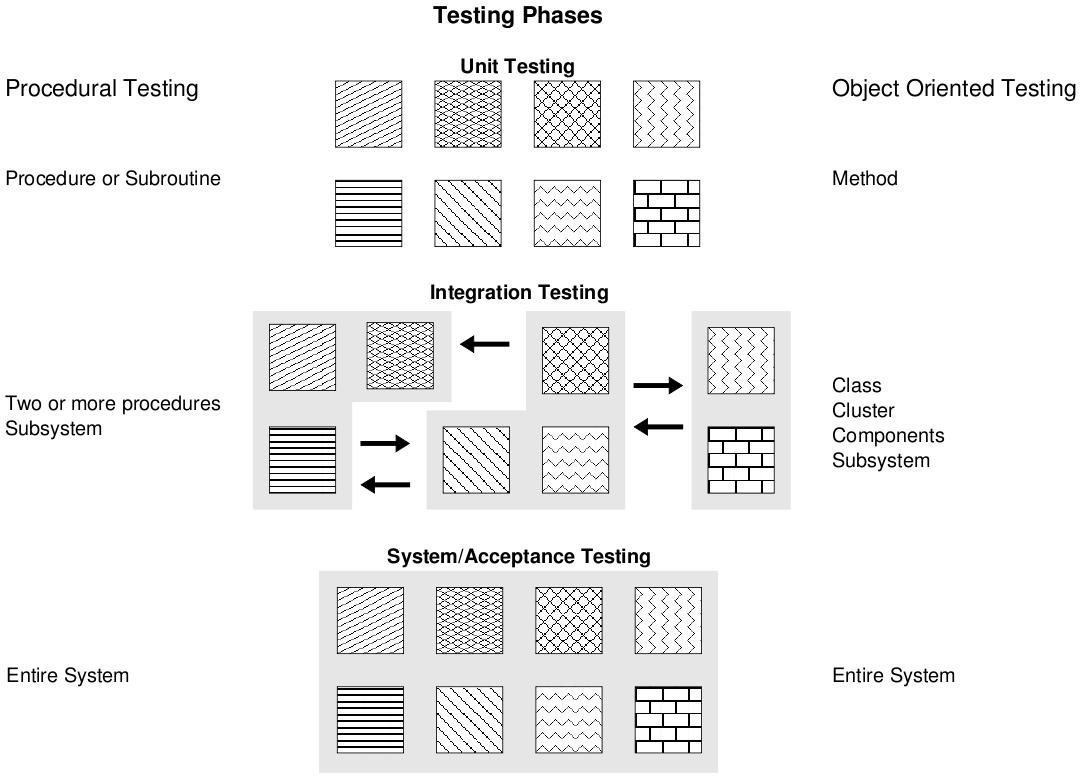
\includegraphics[scale=.3]{test-phases}
\end{block:fact}
\end{frame}


\begin{frame}
\frametitle{Test phases}
\framesubtitle{Unit testing}
\label{concept:unit-testing}

\begin{block:concept}{Definition}
Unit testing verifies the functioning in isolation of software pieces which
are separately testable.
\end{block:concept}

\begin{block:fact}{}
    \centering
    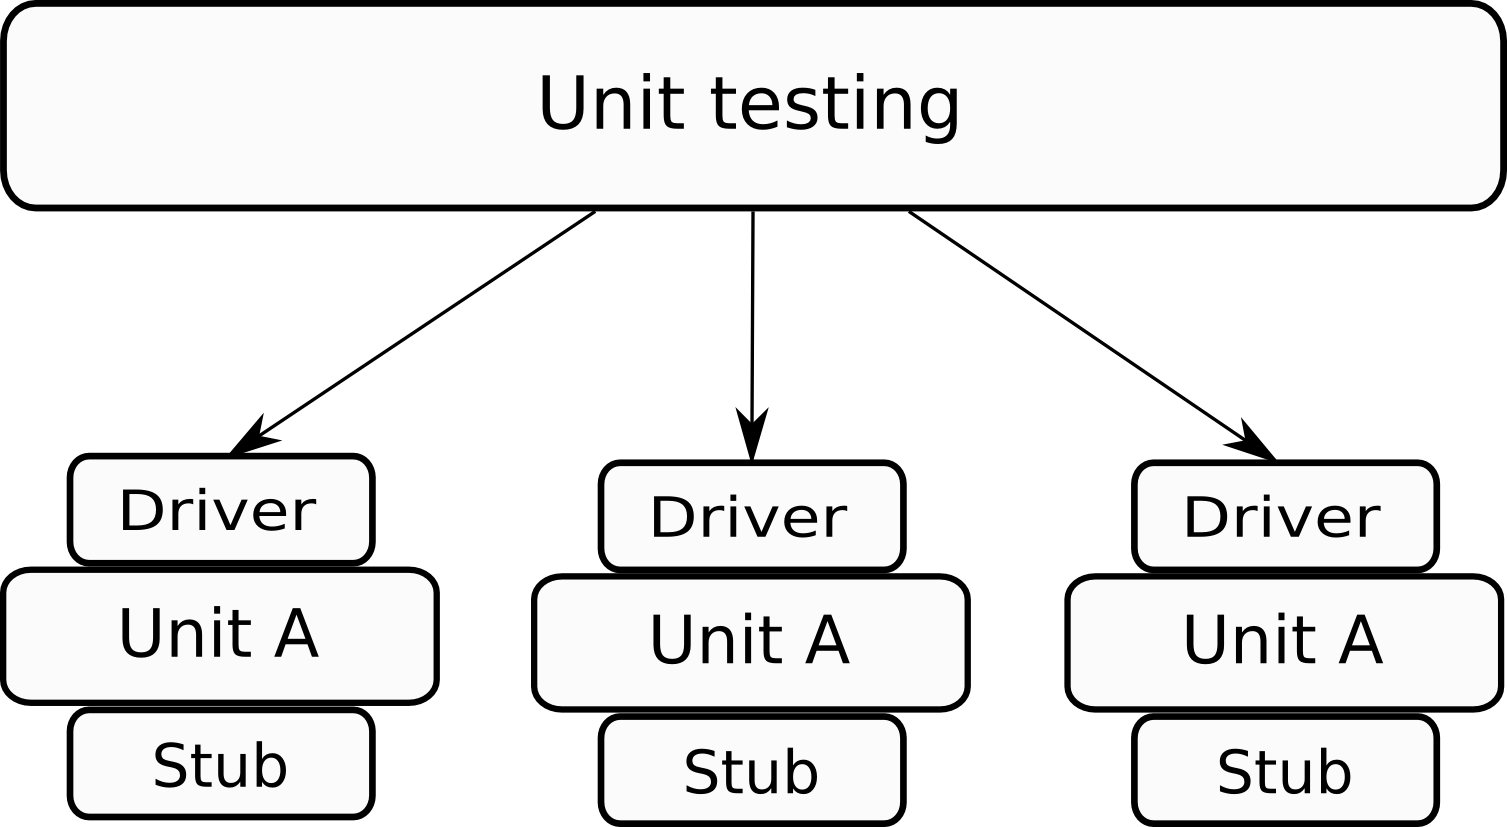
\includegraphics[width=5cm]{unit-testing}
\end{block:fact}

\hfill
\refie{example:pentium-fdiv-bug}{\beamerbutton{Example: Pentium FDIV bug}}
\end{frame}


\begin{frame}
\frametitle{Test phases}
\framesubtitle{Unit testing}

\begin{block:fact}{What is an unit?}
\begin{itemize}
	\item In procedural testing, the unit is the procedure or subroutine.

	\item In object oriented testing, the unit is the method or the class.
	\begin{itemize}
		\item For the time being, we will consider that the unit is the method!
	\end{itemize}
\end{itemize}
\end{block:fact}
\end{frame}



\begin{frame}
\frametitle{Test phases}
\framesubtitle{Unit testing - Stubs}

\begin{block:fact}{How to test an unit?}
\begin{itemize}
	\item Although the definition calls for units that are separately testable,
	this is not always possible.
	\begin{itemize}
		\item Mosts units requires data from other units.
	\end{itemize}

	\item Coupling between units is a threat for unit testing. Thus, it is
	desirable to replace some units by others more simple and predictable
	(just for software testing sake).
\end{itemize}
\end{block:fact}
\end{frame}



\begin{frame}
\frametitle{Test phases}
\framesubtitle{Stubs}
\label{concept:stub}

\begin{block:concept}{Definition}
A stub is a unit that replaces another unit used by the unit under test.
\end{block:concept}

\begin{block:fact}{Why should we use a stub?}
\begin{itemize}
	\item Stubs simulate the behavior of another unit not yet implemented but
	called by the unit under test.

	\item Usually, a stub simulates the expected behavior of the used unit with
	minimum computation effort or data manipulation.
\end{itemize}
\end{block:fact}

\hfill
\refie{example:stub}{\beamerbutton{Example: Stub}}
\end{frame}


\begin{frame}
\frametitle{Test phases}
\framesubtitle{Unit testing - Driver}

\begin{block:fact}{How to test a unit?}
\begin{itemize}
	\item Even tough stubs can be used to replace complex units for a given
	unit under testing, something must setup and wire the stubs into the
	unit.
\end{itemize}
\end{block:fact}
\end{frame}



\begin{frame}
\frametitle{Test phases}
\framesubtitle{Unit testing - Driver}
\label{concept:driver}
\label{concept:test-driver}

\begin{block:concept}{Definition}
Driver is the software responsible for coordinating the testing of a unit.
\end{block:concept}

\begin{block:fact}{What a driver does?}
\begin{itemize}
	\item Drivers are used to test a unit which requires input data provided
	by another unit:
	\begin{enumerate}
		\item it gathers the data provided by the tester,
		\item it passes them to the unit under test in the form of arguments,
		\item it collects the results produced by the unit, and
		\item it shows them to the tester.
	\end{enumerate}
\end{itemize}
\end{block:fact}
\end{frame}


\begin{frame}[c]
\frametitle{Test phases}
\framesubtitle{Unit testing - Driver and stubs}

\begin{block:fact}{}
	\centering
	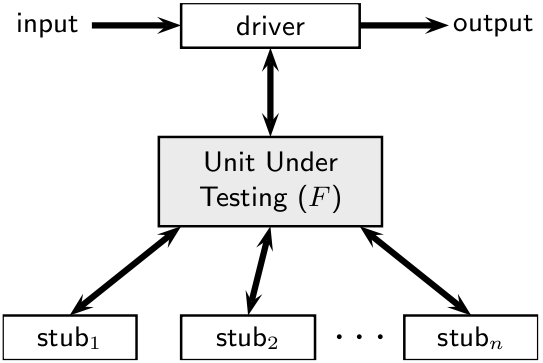
\includegraphics[scale=.3]{driver-and-stub}
\end{block:fact}
\end{frame}



\begin{frame}
\label{concept:integration-testing}
\frametitle{Test phases}
\framesubtitle{Integration testing}

\begin{block:concept}{Definition}
Integration testing verifies whether the units tested individually communicate
accordingly when integrated.
\end{block:concept}

\begin{block:fact}{}
    \centering
    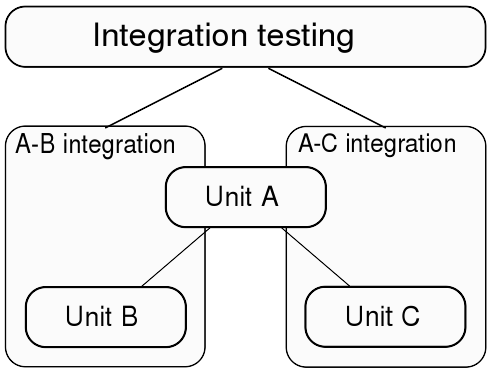
\includegraphics[scale=.3]{integration-testing}
\end{block:fact}

\hfill
\refie{example:mars-climate-orbiter}{\beamerbutton{Example: Mars climate orbiter}}
\end{frame}



\begin{frame}
\frametitle{Test phases}
\framesubtitle{Integration testing}

\begin{block:fact}{Why integration testing is important?}
\begin{itemize}
	\item Integration testing must be performed because:
	\begin{itemize}
		\item Data can be lost at the unit's interface.

		\item Global variables can suffer undesirable interferences.
	\end{itemize}
\end{itemize}
\end{block:fact}

\begin{block:fact}{}
    \centering
    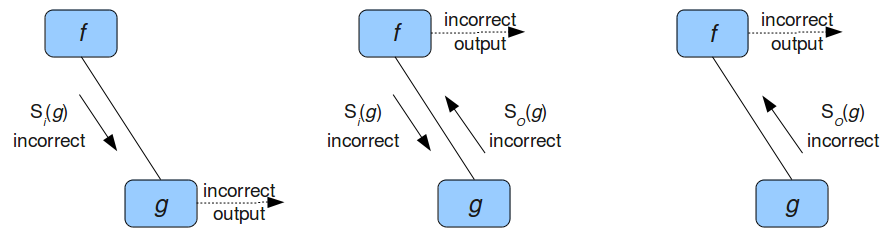
\includegraphics[width=\textwidth]{types-integration-errors}
\end{block:fact}
\end{frame}


\begin{frame}
\label{concept:system-testing}
\frametitle{Test phases}
\framesubtitle{System testing}

\begin{block:concept}{Definition}
System testing ensures that the software and the other elements that
are part of the system (hardware and database, for instance) are adequately
combined and behave as expected.
\end{block:concept}

\begin{block:fact}{Types of system testing}
\begin{itemize}
	\item Typically system testing includes many types of testing:
	\begin{columns}[t, totalwidth=6.5cm]
		\begin{column}[t]{3cm}
			\begin{itemize}
				\item functionality,
				\item usability,
				\item security,
				\item localization,
			\end{itemize}
		\end{column}

		\begin{column}[t]{3cm}
			\begin{itemize}
				\item reliability,
				\item availability,
				\item \ldots
			\end{itemize}
		\end{column}
	\end{columns}
\end{itemize}
\end{block:fact}

\hfill
\refie{example:ghost-train}{\beamerbutton{Example: Ghost train}}
\end{frame}



\begin{frame}[hasprev=true, hasnext=false]
\label{concept:acceptance-testing}
\frametitle{Test phases}
\framesubtitle{Acceptance testing}

\begin{block:concept}{Definition}
Acceptance testing refers to the tester, in general performed by the
user himself, who verifies whether the product satisfies his expectation.
\end{block:concept}

\begin{block:fact}{Alpha/Beta testing}
\begin{itemize}
	\item Informally, it can be defined alpha and beta testing.
	\begin{itemize}
		\item Alpha testing: software is installed and used internally (in the
		company that developed).

		\item Beta testing: software is installed and tested by external
		users.
	\end{itemize}
\end{itemize}
\end{block:fact}

\begin{block:fact}{Why is acceptance testing important?}
\begin{itemize}
    \item Acceptance testing, when completed successfully, will result in the
    customer accepting the software.
\end{itemize}
\end{block:fact}
\end{frame}